\let\negmedspace\undefined
\let\negthickspace\undefined
\documentclass[journal,12pt,onecolumn]{IEEEtran}
\usepackage{cite}
\usepackage{amsmath,amssymb,amsfonts,amsthm}
\usepackage{algorithmic}
\usepackage{graphicx}
\graphicspath{{./figs/}}
\usepackage{textcomp}
\usepackage{xcolor}
\usepackage{txfonts}
\usepackage{listings}
\usepackage{enumitem}
\usepackage{mathtools}
\usepackage{gensymb}
\usepackage{comment}
\usepackage{caption}
\usepackage[breaklinks=true]{hyperref}
\usepackage{tkz-euclide} 
\usepackage{listings}
\usepackage{gvv}                                        
%\def\inputGnumericTable{}                                 
\usepackage[latin1]{inputenc}     
\usepackage{xparse}
\usepackage{color}                                            
\usepackage{array}
\usepackage{longtable}                                       
\usepackage{calc}                                             
\usepackage{multirow}
\usepackage{multicol}
\usepackage{hhline}                                           
\usepackage{ifthen}                                           
\usepackage{lscape}
\usepackage{tabularx}
\usepackage{array}
\usepackage{float}
\newtheorem{theorem}{Theorem}[section]
\newtheorem{problem}{Problem}
\newtheorem{proposition}{Proposition}[section]
\newtheorem{lemma}{Lemma}[section]
\newtheorem{corollary}[theorem]{Corollary}
\newtheorem{example}{Example}[section]
\newtheorem{definition}[problem]{Definition}
\newcommand{\BEQA}{\begin{eqnarray}}
\newcommand{\EEQA}{\end{eqnarray}}
\newcommand{\define}{\stackrel{\triangle}{=}}
\theoremstyle{remark}
\newtheorem{rem}{Remark}

\begin{document}

\title{5.2.58}
\author{ee25btech11056 - Suraj.N}
\maketitle
\renewcommand{\thefigure}{\theenumi}
\renewcommand{\thetable}{\theenumi}

\begin{document}

\textbf{Question :} Solve the system of equations
\[
\begin{aligned}
x - y + z &= 4\\
2x + y - 3z &= 0\\
x + y + z &= 2
\end{aligned}
\]

\textbf{Solution :}

\begin{table}[h!]
  \centering
  \begin{table}[h!]
    \centering
    \begin{tabular}{|c|c|}
        \hline
        Point & Coordinates \\
        \hline
	    $A$ & $\myvec{1\\-1}$ \\
	    $B$ & $\myvec{-4\\2k}$ \\
	    $C$ & $\myvec{-k\\-5}$ \\
        \hline
    \end{tabular}
    \caption{Vertices of $\triangle ABC$ before substituting $k$}
    \label{tab:triangle_k}
\end{table}

  \caption*{Table : Equations}
  \label{5.2.58}
\end{table}

The system of equations in matrix form is :

\begin{align}
  \myvec{1 & -1 & 1\\2 & 1 & -3\\1 & 1 & 1}\myvec{x\\y\\z} &= \myvec{4\\0\\2}
\end{align}

Forming the augmented matrix,

\begin{align}
  \myaugvec{3}{1 & -1 & 1 & 4\\ 2 & 1 & -3 & 0\\1 & 1 & 1 & 2}
\end{align}

Using Gaussian elimination,

\begin{align}
  \myaugvec{3}{1 & -1 & 1 & 4\\ 2 & 1 & -3 & 0\\1 & 1 & 1 & 2}
  \xleftrightarrow[\;R_2 \to R_2 -2R_1\;]{\;R_3 \to R_3 - R_1}
  \myaugvec{3}{1 & -1 & 1 & 4\\0 & 3 & -5 & -8\\0 & 2 & 0 & -2}
  \xleftrightarrow{R_3 \to R_3 -\tfrac{2}{3}R_2}
  \myaugvec{3}{1 & -1 & 1 & 4\\0 & 3 & -5 & -8\\0 & 0 & \tfrac{10}{3} & \tfrac{10}{3}}
\end{align}

Using back substitution we get :

\begin{align}
  \tfrac{10}{3} z &= \tfrac{10}{3}\\ 
  z &= 1\\
  3y - 5z &= -8\\
  3y - 5 &= -8\\
  3y &= -3\\
  y &= -1\\
  x - y + z &= 4\\
  x + 2 &= 4\\
  x &= 2
\end{align}

\pagebreak

Therefore the solution for the system of equations is : 

\begin{align}
  \myvec{2\\-1\\1}
\end{align}





\pagebreak

\begin{figure}[h!]
  \centering
  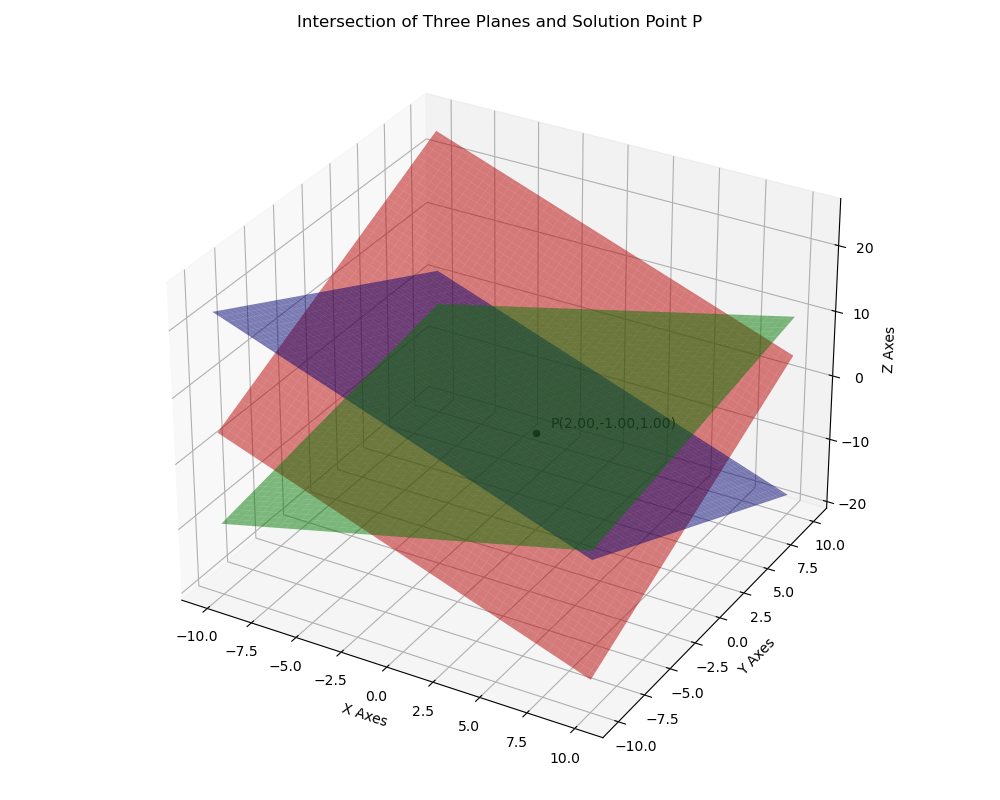
\includegraphics[width=0.7\columnwidth]{figs/solution.png} 
   \caption*{Fig : Planes}
  \label{Fig1}
\end{figure}


\end{document}

